\documentclass[border=3pt]{standalone}
% Preâmbulo compartilhado pelos diagramas TikZ da aula 13 (SLAM com EKF)
\usepackage[T1]{fontenc}
\usepackage[utf8]{inputenc}
\usepackage{lmodern}
\usepackage{amsmath}
\usepackage{xcolor}
\usepackage{tikz}
\usetikzlibrary{arrows.meta,angles,quotes,decorations.pathmorphing,decorations.pathreplacing,calc,
                positioning,shapes.geometric,shapes.misc,backgrounds,fit,
                math}

% Paleta (mesma dos SVGs originais)
\definecolor{dblue}{HTML}{2A5B8C}
\definecolor{dorange}{HTML}{B3541E}
\definecolor{dgreen}{HTML}{4A7C59}
\definecolor{dred}{HTML}{9C4B4B}
\definecolor{dcream}{HTML}{F4F1EA}
\definecolor{dshade}{HTML}{DDD7C9}

% Função gaussiana (não normalizada por padrão de escala visual)
\pgfmathdeclarefunction{gauss}{3}{%
  \pgfmathparse{1/(#3*sqrt(2*pi))*exp(-((#1-#2)^2)/(2*#3^2))}%
}

% Estilos comuns (prefixo d... para não colidir com chaves internas do pgf)
\tikzset{
  >={Stealth[length=2mm]},
  dguide/.style={gray!55, dashed, line width=0.4pt},
  daxis/.style={gray!60, line width=0.7pt, ->},
  dbody/.style={fill=black!3, draw=black!80, line width=1pt},
  dacc/.style={draw=dblue, line width=1pt},
  dlbl/.style={black!55, font=\small},
  dsub/.style={black!45, font=\footnotesize},
  dstate/.style={circle, draw=black!80, fill=dcream, line width=1pt,
                 minimum size=17mm, font=\large, inner sep=1pt},
  dobs/.style={circle, draw=black!80, fill=dshade, line width=1pt,
               minimum size=14mm, font=\large, inner sep=1pt},
  dbox/.style={rounded corners=2pt, draw=black!80, fill=dcream, line width=1pt,
               align=center, inner sep=6pt},
  dop/.style={circle, draw=black!80, fill=white, line width=1pt,
              minimum size=6mm, inner sep=0pt, font=\small},
  dtrans/.style={->, dblue, line width=1pt},
  dmeas/.style={->, dorange, line width=1pt},
  dcurve/.style={line width=1pt, dblue},
  dcurveb/.style={line width=1.4pt, dorange},
}

\begin{document}
\hyphenpenalty=10000 \exhyphenpenalty=10000 \tolerance=9999 \emergencystretch=3em
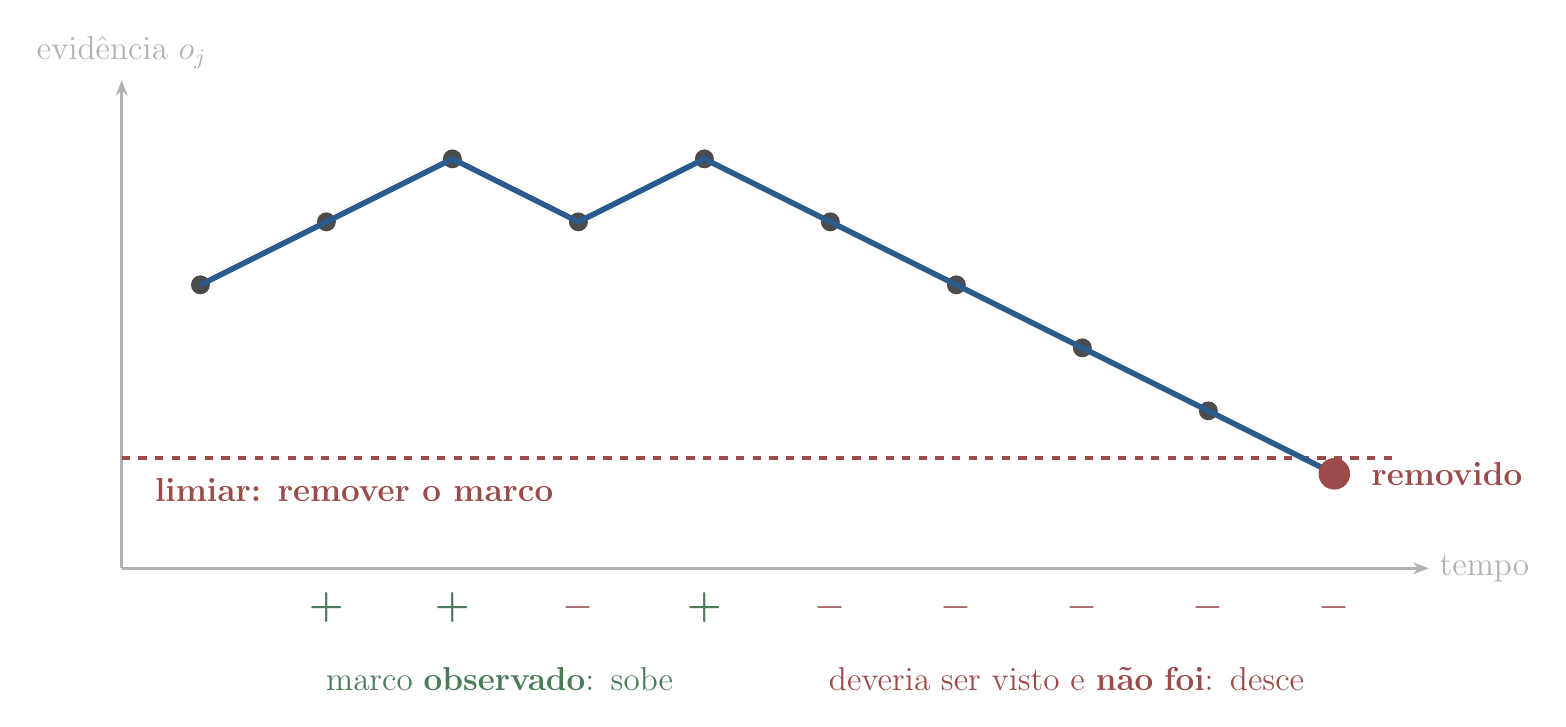
\begin{tikzpicture}[x=1cm,y=1cm]
\draw[daxis, line width=1.2pt] (1.2,1.6) -- (17.8,1.6) node[right, font=\large] {tempo};
\draw[daxis, line width=1.2pt] (1.2,1.6) -- (1.2,7.8) node[above, font=\large] {evidência $o_j$};
\draw[dred, dashed, line width=1.6pt] (1.2,3.0) -- (17.4,3.0);
\node[font=\large\bfseries, dred, anchor=west] at (1.5,2.6) {limiar: remover o marco};
\foreach \i/\v in {0/5.2,1/6.0,2/6.8,3/6.0,4/6.8,5/6.0,6/5.2,7/4.4,8/3.6,9/2.8} {
  \fill[black!70] ({2.2+\i*1.6},\v) circle (0.12);
}
\draw[dblue, line width=2pt] (2.2,5.2) -- (3.8,6.0) -- (5.4,6.8) -- (7.0,6.0) -- (8.6,6.8) -- (10.2,6.0) -- (11.8,5.2) -- (13.4,4.4) -- (15.0,3.6) -- (16.6,2.8);
\foreach \i/\t/\c in {1/{+}/dgreen,2/{+}/dgreen,3/{$-$}/dred,4/{+}/dgreen,5/{$-$}/dred,6/{$-$}/dred,7/{$-$}/dred,8/{$-$}/dred,9/{$-$}/dred} {
  \node[font=\Large\bfseries, text=\c] at ({2.2+\i*1.6},1.1) {\t};
}
\node[font=\large, dgreen, text width=5cm, align=center] at (6.0,0.2) {marco \textbf{observado}: sobe};
\node[font=\large, dred, text width=7cm, align=center] at (13.2,0.2) {deveria ser visto e \textbf{não foi}: desce};
\fill[dred] (16.6,2.8) circle (0.2); \node[font=\large\bfseries, dred, anchor=west] at (16.95,2.8) {removido};
\end{tikzpicture}
\end{document}
